\documentclass[12pt]{article}

\usepackage{amsmath, mathtools}
\usepackage{amsfonts}
\usepackage{amssymb}
\usepackage{graphicx}
\usepackage{colortbl}
\usepackage{xr}
\usepackage{hyperref}
\usepackage{longtable}
\usepackage{xfrac}
\usepackage{tabularx}
\usepackage{float}
\usepackage{siunitx}
\usepackage{booktabs}
\usepackage{caption}
\usepackage{pdflscape}
\usepackage{afterpage}
\usepackage{enumitem}

\usepackage[round]{natbib}

%\usepackage{refcheck}

\hypersetup{
    bookmarks=true,         % show bookmarks bar?
    colorlinks=true,        % false: boxed links; true: colored links
    linkcolor=red,          % color of internal links (change box color with linkbordercolor)
    citecolor=green,        % color of links to bibliography
    filecolor=magenta,      % color of file links
    urlcolor=cyan           % color of external links
}

\usepackage{fullpage}

%% Comments

\usepackage{color}

\newif\ifcomments\commentstrue %displays comments
%\newif\ifcomments\commentsfalse %so that comments do not display

\ifcomments
\newcommand{\authornote}[3]{\textcolor{#1}{[#3 ---#2]}}
\newcommand{\todo}[1]{\textcolor{red}{[TODO: #1]}}
\else
\newcommand{\authornote}[3]{}
\newcommand{\todo}[1]{}
\fi

\newcommand{\wss}[1]{\authornote{blue}{SS}{#1}} 
\newcommand{\plt}[1]{\authornote{magenta}{TPLT}{#1}} %For explanation of the template
\newcommand{\an}[1]{\authornote{cyan}{Author}{#1}}

%% Common Parts

\newcommand{\progname}{SFWRENG 4G06} % PUT YOUR PROGRAM NAME HERE
\newcommand{\authname}{Team 9, dice\_devs
\\ John Popovici
\\ Nigel Moses
\\ Naishan Guo
\\ Hemraj Bhatt
\\ Isaac Giles} % AUTHOR NAMES                  

\usepackage{hyperref}
    \hypersetup{colorlinks=true, linkcolor=blue, citecolor=blue, filecolor=blue,
                urlcolor=blue, unicode=false}
    \urlstyle{same}
                                

% For easy change of table widths
\newcommand{\colZwidth}{1.0\textwidth}
\newcommand{\colAwidth}{0.13\textwidth}
\newcommand{\colBwidth}{0.82\textwidth}
\newcommand{\colCwidth}{0.1\textwidth}
\newcommand{\colDwidth}{0.05\textwidth}
\newcommand{\colEwidth}{0.8\textwidth}
\newcommand{\colFwidth}{0.17\textwidth}
\newcommand{\colGwidth}{0.5\textwidth}
\newcommand{\colHwidth}{0.28\textwidth}

% Used so that cross-references have a meaningful prefix
\newcounter{defnum} %Definition Number
\newcommand{\dthedefnum}{GD\thedefnum}
\newcommand{\dref}[1]{GD\ref{#1}}
\newcounter{datadefnum} %Datadefinition Number
\newcommand{\ddthedatadefnum}{DD\thedatadefnum}
\newcommand{\ddref}[1]{DD\ref{#1}}
\newcounter{theorynum} %Theory Number
\newcommand{\tthetheorynum}{TM\thetheorynum}
\newcommand{\tref}[1]{TM\ref{#1}}
\newcounter{tablenum} %Table Number
\newcommand{\tbthetablenum}{TB\thetablenum}
\newcommand{\tbref}[1]{TB\ref{#1}}
\newcounter{assumpnum} %Assumption Number
\newcommand{\atheassumpnum}{A\theassumpnum}
\newcommand{\aref}[1]{A\ref{#1}}
\newcounter{goalnum} %Goal Number
\newcommand{\gthegoalnum}{GS\thegoalnum}
\newcommand{\gsref}[1]{GS\ref{#1}}
\newcounter{instnum} %Instance Number
\newcommand{\itheinstnum}{IM\theinstnum}
\newcommand{\iref}[1]{IM\ref{#1}}
\newcounter{reqnum} %Requirement Number
\newcommand{\rthereqnum}{R\thereqnum}
\newcommand{\rref}[1]{R\ref{#1}}
\newcounter{nfrnum} %NFR Number
\newcommand{\rthenfrnum}{NFR\thenfrnum}
\newcommand{\nfrref}[1]{NFR\ref{#1}}
\newcounter{lcnum} %Likely change number
\newcommand{\lthelcnum}{LC\thelcnum}
\newcommand{\lcref}[1]{LC\ref{#1}}
\newcommand{\deftheory}[9][Not Applicable]
{
\newpage
\noindent \rule{\textwidth}{0.5mm}

\paragraph{RefName: } \textbf{#2} \phantomsection 
\label{#2}

\paragraph{Label:} #3

\noindent \rule{\textwidth}{0.5mm}

\paragraph{Equation:}

#4

\paragraph{Description:}

#5

\paragraph{Notes:}

#6

\paragraph{Source:}

#7

\paragraph{Ref.\ By:}

#8

\paragraph{Preconditions for \hyperref[#2]{#2}:}
\label{#2_precond}

#9

\paragraph{Derivation for \hyperref[#2]{#2}:}
\label{#2_deriv}

#1

\noindent \rule{\textwidth}{0.5mm}

}

\begin{document}

\title{Software Requirements Specification for\\\progname:\\Dice Duels: Duel of the Eights} 
\author{\authname}
\date{\today}
	
\maketitle

~\newpage

\pagenumbering{roman}

\tableofcontents

~\newpage

% revision history
\section*{Revision History}

\begin{table}[hp]
\caption{Revision History} \label{TblRevisionHistory}
\begin{tabularx}{\textwidth}{llX}
\toprule
\textbf{Date} & \textbf{Developer(s)} & \textbf{Change}\\
\midrule
2024-09-27 & John Popovici & Set up formatting\\
2024-09-30 & Nigel Moses & Added three blank sections (Commonalities related sections)\\
2024-10-05 & John Popovici & Added content to section 4.1 and 4.1.1\\
\dots & \dots & \dots\\
\bottomrule
\end{tabularx}
\end{table}

%~\\
%\plt{This template is intended for use by CAS 741.  For CAS 741 the template should be used exactly as given, except the Reflection Appendix can be deleted. For the capstone course it is a source of ideas, but shouldn't be followed exactly.  The exception is the reflection appendix.  All capstone SRS documents should have a refelection appendix.}

% section 1: reference material
\section{Reference Material}

%This section records information for easy reference.\\

This section has been simplified due to the simplistic nature of our problem space. No unit symbols are used in our document and anywhere a unit is used, it is stated. Additionally all abbreviations and acronyms are explained where they first appear in the document and are from there on out self-explanatory and contextually understandable. There are also no mathematical formulas or mathematical notation within our software requirements specification document. This document was compiled for the SFWRENG 4G06 course, the software engineering capstone course at McMaster University.

\subsection{Symbols, Abbreviations, and Acronyms}

\begin{table}[H]
\begin{tabular}{l l} 
  \toprule		
  \textbf{symbol} & \textbf{description}\\
  \midrule
  SFWRENG 4G06 & Program Capstone Course\\
  SRS & Software Requirements Specification\\
  X in AdXrB & number of dice faces\\
  A in AdXrB & number of dice\\
  B in AdXrB & number of dice rolls\\
  GSX & Goal statement number X\\
  SGX & Stretch goal number X\\
  RX & Functional Requirement number X\\
  NFRX & Non-Functional Requirement number X\\
  LCX & Likely Change number X\\
  UCX & Unlikely Change number X\\
  UI & User Interface\\
  CPU & Central Processing Unit\\
  GPU & Graphics Processing Unit\\
  PC & Personal Computer\\
  UI & User Interface\\
  UX & User Experience\\
  3D & Three dimensional\\
  OS & Operating System\\
  ms & milliseconds\\
  FPS & Frames Per Second\\
  PvP & Player versus Player\\
  GDPR & General Data Protection Regulation\\
  CCPA & California Consumer Privacy Act\\
  COPPA & Children’s Online Privacy Protection Act\\
  IEEE & Institute of Electrical and Electronics Engineers\\
  LAN & Local Area Network\\
  RFC & Request For Comments\\
  ISO & International Organization for Standardization\\
  IEC & International Electrotechnical Commission\\
  EULA & End-User License Agreement\\
  ESRB & Entertainment Software Rating Board\\
  PEGI & Pan European Game Information\\
  WCAG & Web Content Accessibility Guidelines\\
  

  \bottomrule
  
\end{tabular}\\
\caption{Table of Symbols, Abbreviations, and Acronyms}
\end{table}
% \plt{Add any other abbreviations or acronyms that you add}









\iffalse
\subsection{Table of Units}

Throughout this document SI (Syst\`{e}me International d'Unit\'{e}s) is employed
as the unit system.  In addition to the basic units, several derived units are
used as described below.  For each unit, the symbol is given followed by a
description of the unit and the SI name.
~\newline

\renewcommand{\arraystretch}{1.2}
%\begin{table}[ht]
  \noindent \begin{tabular}{l l l} 
    \toprule		
    \textbf{symbol} & \textbf{unit} & \textbf{SI}\\
    \midrule 
    \si{\metre} & length & metre\\
    \si{\kilogram} & mass	& kilogram\\
    \si{\second} & time & second\\
    \si{\celsius} & temperature & centigrade\\
    \si{\joule} & energy & joule\\
    \si{\watt} & power & watt (W = \si{\joule\per\second})\\
    \bottomrule
  \end{tabular}
  %	\caption{Provide a caption}
%\end{table}

\plt{Only include the units that your SRS actually uses.}

\plt{Derived units, like newtons, pascal, etc, should show their derivation
    (the units they are derived from) if their constituent units are in the
    table of units (that is, if the units they are derived from are used in the
    document).  For instance, the derivation of pascals as
    $\si{\pascal}=\si{\newton\per\square\meter}$ is shown if newtons and m are
    both in the table.  The derivations of newtons would not be shown if kg and
    s are not both in the table.}

\plt{The symbol for units named after people use capital letters, but the name
  of the unit itself uses lower case.  For instance, pascals use the symbol Pa,
  watts use the symbol W, teslas use the symbol T, newtons use the symbol N,
  etc.  The one exception to this is degree Celsius.  Details on writing metric
  units can be found on the 
  \href{https://www.nist.gov/pml/weights-and-measures/writing-metric-units}
  {NIST} web-page.}

\subsection{Table of Symbols}

The table that follows summarizes the symbols used in this document along with
their units.  The choice of symbols was made to be consistent with the heat
transfer literature and with existing documentation for solar water heating
systems.  The symbols are listed in alphabetical order.

\renewcommand{\arraystretch}{1.2}
%\noindent \begin{tabularx}{1.0\textwidth}{l l X}
\noindent \begin{longtable*}{l l p{12cm}} \toprule
\textbf{symbol} & \textbf{unit} & \textbf{description}\\
\midrule 
$A_C$ & \si[per-mode=symbol] {\square\metre} & coil surface area
\\
$A_\text{in}$ & \si[per-mode=symbol] {\square\metre} & surface area over 
which heat is transferred in
\\ 
\bottomrule
\end{longtable*}
\plt{Use your problems actual symbols.  The si package is a good idea to use for
  units.}

\subsection{Abbreviations and Acronyms}

\renewcommand{\arraystretch}{1.2}
\begin{tabular}{l l} 
  \toprule		
  \textbf{symbol} & \textbf{description}\\
  \midrule 
  A & Assumption\\
  DD & Data Definition\\
  GD & General Definition\\
  GS & Goal Statement\\
  IM & Instance Model\\
  LC & Likely Change\\
  PS & Physical System Description\\
  R & Requirement\\
  SRS & Software Requirements Specification\\
  \progname{} & \plt{put an expanded version of your program name here (as appropriate)}\\
  TM & Theoretical Model\\
  \bottomrule
\end{tabular}\\

\plt{Add any other abbreviations or acronyms that you add}

\subsection{Mathematical Notation}

\plt{This section is optional, but should be included for projects that make use
  of notation to convey mathematical information.  For instance, if typographic
  conventions (like bold face font) are used to distinguish matrices, this
  should be stated here.  If symbols are used to show mathematical operations,
  these should be summarized here.  In some cases the easiest way to summarize
  the notation is to point to a text or other source that explains the
  notation.}

\plt{This section was added to the template because some students use very
  domain specific notation.  This notation will not be readily understandable to
  people outside of your domain.  It should be explained.}
\fi

\pagenumbering{arabic}
% comments - to be commented out
% \plt{This SRS template is based on \citet{SmithAndLai2005, SmithEtAl2007,
  SmithAndKoothoor2016}.  It will get you started.  You should not modify the
  section headings, without first discussing the change with the course
  instructor.  Modification means you are not following the template, which
  loses some of the advantage of a template, especially standardization.
  Although the bits shown below do not include type information, you may need to
  add this information for your problem.  If you are unsure, please can ask the
  instructor.}

\plt{Feel free to change the appearance of the report by modifying the LaTeX
  commands.}

\plt{This template document assumes that a single program is being documented.
  If you are documenting a family of models, you should start with a commonality
  analysis.  A separate template is provided for this.  For program
  families you should look at \cite{Smith2006, SmithMcCutchanAndCarette2017}.
  Single family member programs are often programs based on a single physical
  model.  General purpose tools are usually documented as a family.  Families of
  physical models also come up.}

\plt{The SRS is not generally written, or read, sequentially.  The SRS is a
  reference document.  It is generally read in an ad hoc order, as the need
  arises.  For writing an SRS, and for reading one for the first time, the
  suggested order of sections is:
\begin{itemize}
\item Goal Statement
\item Instance Models
\item Requirements
\item Introduction
\item Specific System Description
\end{itemize}
}

\plt{Guiding principles for the SRS document:
\begin{itemize}
\item Do not repeat the same information at the same abstraction level.  If
  information is repeated, the repetition should be at a different abstraction
  level.  For instance, there will be overlap between the scope section and the
  assumptions, but the scope section will not go into as much detail as the
  assumptions section.
\end{itemize}
}

\plt{The template description comments should be disabled before submitting this
  document for grading.}

\plt{You can borrow any wording from the text given in the template.  It is part
  of the template, and not considered an instance of academic integrity.  Of
  course, you need to cite the source of the template.}

\plt{When the documentation is done, it should be possible to trace back to the
  source of every piece of information.  Some information will come from
  external sources, like terminology.  Other information will be derived, like
  General Definitions.}

\plt{An SRS document should have the following qualities: unambiguous,
  consistent, complete, validatable, abstract and traceable.}

\plt{The overall goal of the SRS is that someone that meets the Characteristics
  of the Intended Reader (Section~\ref{sec_IntendedReader}) can learn,
  understand and verify the captured domain knowledge.  They should not have to
  trust the authors of the SRS on any statements.  They should be able to
  independently verify/derive every statement made.}

% section 2: Introduction
% section 3: General System Description
\section{Introduction}

\plt{The introduction section is written to introduce the problem.  It starts
  general and focuses on the problem domain. The general advice is to start with
a paragraph or two that describes the problem, followed by a ``roadmap''
paragraph.  A roadmap orients the reader by telling them what sub-sections to
expect in the Introduction section.}

\subsection{Purpose of Document}

\plt{This section summarizes the purpose of the SRS document.  It does not focus
  on the problem itself.  The problem is described in the ``Problem
  Description'' section (Section~\ref{Sec_pd}).  The purpose is for the document
  in the context of the project itself, not in the context of this course.
  Although the ``purpose'' of the document is to get a grade, you should not
  mention this.  Instead, ``fake it'' as if this is a real project.  The purpose
  section will be similar between projects.  The purpose of the document is the
  purpose of the SRS, including communication, planning for the design stage,
  etc.}

\subsection{Scope of Requirements} 

\plt{Modelling the real world requires simplification.  The full complexity of
  the actual physics, chemistry, biology is too much for existing models, and
  for existing computational solution techniques.  Rather than say what is in
  the scope, it is usually easier to say what is not.  You can think of it as
  the scope is initially everything, and then it is constrained to create the
  actual scope.  For instance, the problem can be restricted to 2 dimensions, or
  it can ignore the effect of temperature (or pressure) on the material
  properties, etc.}  

\plt{The scope section is related to the assumptions section
  (Section~\ref{sec_assumpt}).  However, the scope and the assumptions are not
  at the same level of abstraction.  The scope is at a high level.  The focus is
  on the ``big picture'' assumptions.  The assumptions section lists, and
  describes, all of the assumptions.}

\plt{The scope section is relevant for later determining typical values of inputs. The scope should make it clear what inputs are reasonable to expect. This is a distinction between scope and context (context is a later section).  Scope affects the inputs while context affects how the software will be used.}

\subsection{Characteristics of Intended Reader} \label{sec_IntendedReader}

\plt{This section summarizes the skills and knowledge of the readers of the
  SRS.  It does NOT have the same purpose as the ``User Characteristics''
  section (Section~\ref{SecUserCharacteristics}).  The intended readers are the
  people that will read, review and maintain the SRS.  They are the people that
  will conceivably design the software that is intended to meet the
  requirements.  The user, on the other hand, is the person that uses the
  software that is built.  They may never read this SRS document.  Of course,
  the same person could be a ``user'' and an ``intended reader.''}

\plt{The intended reader characteristics should be written as unambiguously and
  as specifically as possible.  Rather than say, the user should have an
  understanding of physics, say what kind of physics and at what level.  For
  instance, is high school physics adequate, or should the reader have had a
  graduate course on advanced quantum mechanics?}

\subsection{Organization of Document}

\plt{This section provides a roadmap of the SRS document.  It will help the
  reader orient themselves.  It will provide direction that will help them
  select which sections they want to read, and in what order.  This section will
  be similar between project.}

\newpage
\section{General System Description}

This section provides general information about the system.  It identifies the
interfaces between the system and its environment, describes the user
characteristics and lists the system constraints.  \plt{This text can likely be
  borrowed verbatim.}

\plt{The purpose of this section is to provide general information about the
  system so the specific requirements in the next section will be easier to
  understand. The general system description section is designed to be
  changeable independent of changes to the functional requirements documented in
  the specific system description. The general system description provides a
  context for a family of related models.  The general description can stay the
  same, while specific details are changed between family members.}

\subsection{System Context}

\plt{Your system context will include a figure that shows the abstract view of
  the software.  Often in a scientific context, the program can be viewed
  abstractly following the design pattern of Inputs $\rightarrow$ Calculations
  $\rightarrow$ Outputs.  The system context will therefore often follow this
  pattern.  The user provides inputs, the system does the calculations, and then
  provides the outputs to the user.  The figure should not show all of the
  inputs, just an abstract view of the main categories of inputs (like material
  properties, geometry, etc.).  Likewise, the outputs should be presented from
  an abstract point of view.  In some cases the diagram will show other external
  entities, besides the user.  For instance, when the software product is a
  library, the user will be another software program, not an actual end user.
  If there are system constraints that the software must work with external
  libraries, these libraries can also be shown on the System Context diagram.
  They should only be named with a specific library name if this is required by
  the system constraint.}

\begin{figure}[h!]
\begin{center}
 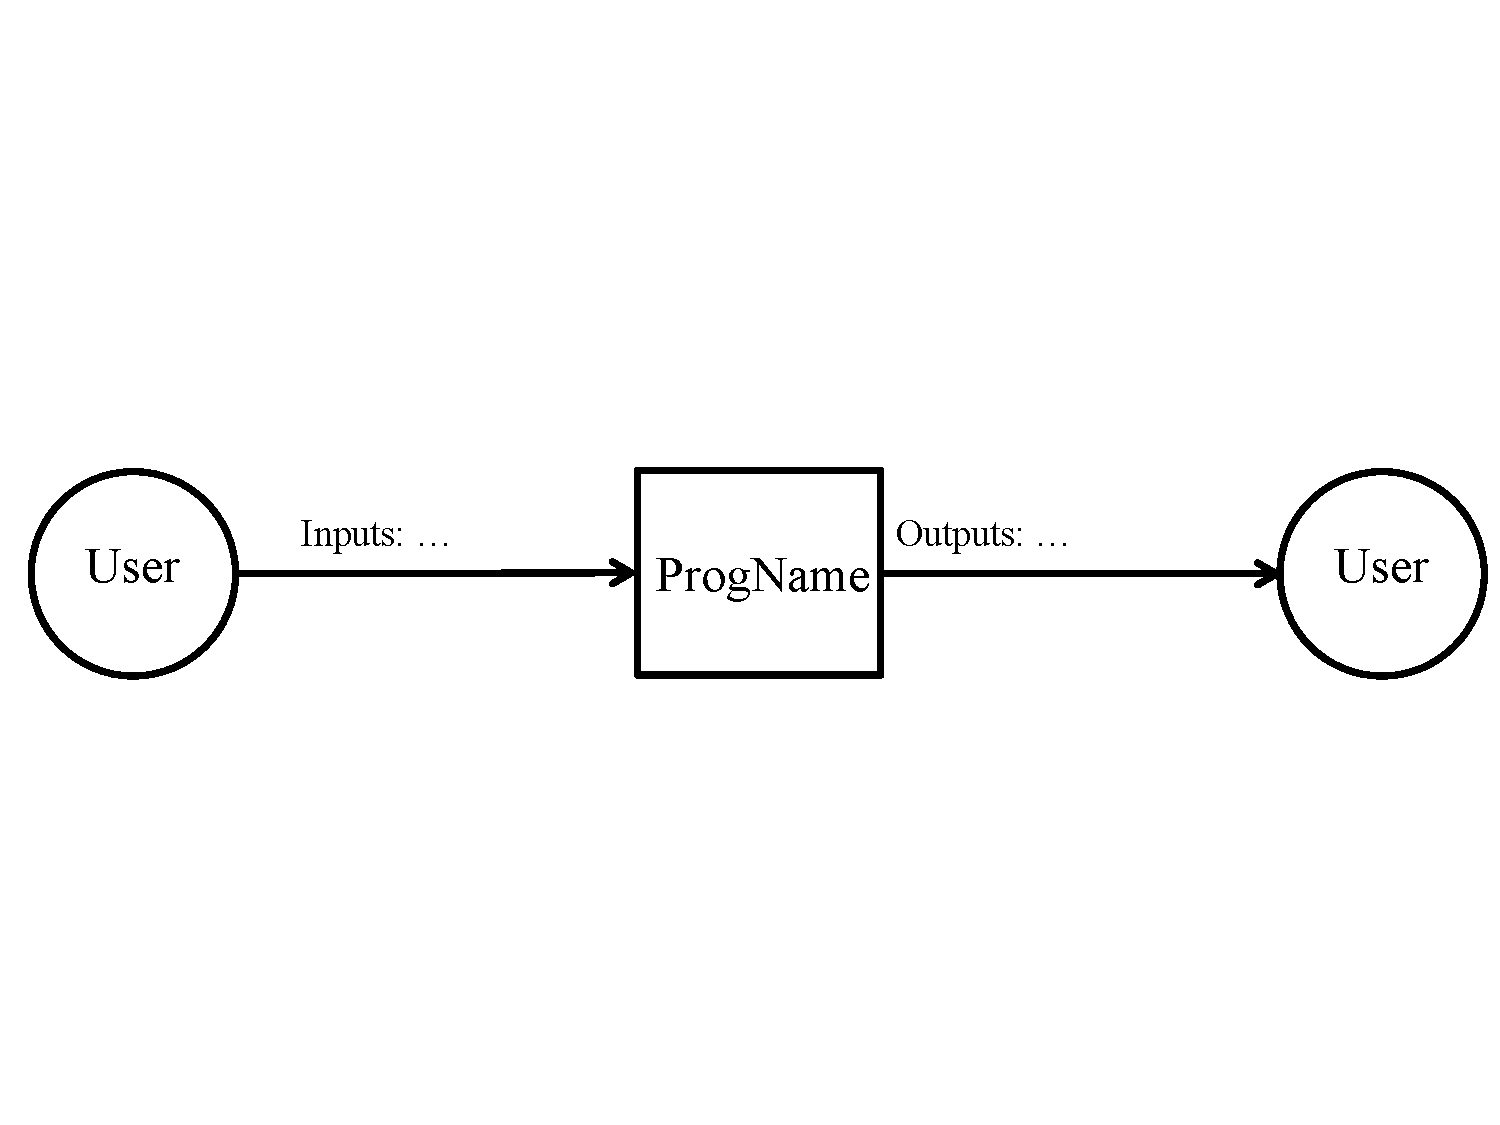
\includegraphics[width=0.6\textwidth]{figures/SystemContextFigure}
\caption{System Context}
\label{Fig_SystemContext} 
\end{center}
\end{figure}

\plt{For each of the entities in the system context diagram its responsibilities
  should be listed.  Whenever possible the system should check for data quality,
  but for some cases the user will need to assume that responsibility.  The list
  of responsibilities should be about the inputs and outputs only, and they
  should be abstract.  Details should not be presented here.  However, the
  information should not be so abstract as to just say ``inputs'' and
  ``outputs''.  A summarizing phrase can be used to characterize the inputs.
  For instance, saying ``material properties'' provides some information, but it
  stays away from the detail of listing every required properties.}

\begin{itemize}
\item User Responsibilities:
\begin{itemize}
\item 
\end{itemize}
\item \progname{} Responsibilities:
\begin{itemize}
\item Detect data type mismatch, such as a string of characters instead of a
  floating point number
\item 
\end{itemize}
\end{itemize}

\plt{Identify in what context the software will typically be used.  Is it for
exploration? education? engineering work? scientific work?. Identify whether it
will be used for mission-critical or safety-critical applications.} \plt{This
additional context information is needed to determine how much effort should be
devoted to the rationale section.  If the application is safety-critical, the
bar is higher.  This is currently less structured, but analogous to, the idea to
the Automotive Safety Integrity Levels (ASILs) that McSCert uses in their
automotive hazard analyses.}

\wss{The }
\subsection{User Characteristics} \label{SecUserCharacteristics}

\plt{This section summarizes the knowledge/skills expected of the user.
  Measuring usability, which is often a required non-function requirement,
  requires knowledge of a typical user.  As mentioned above, the user is a
  different role from the ``intended reader,'' as given in
  Section~\ref{sec_IntendedReader}.  As in Section~\ref{sec_IntendedReader}, the
  user characteristics should be specific an unambiguous.  For instance, ``The
  end user of \progname{} should have an understanding of undergraduate Level 1
  Calculus and Physics.''}

\subsection{System Constraints}

\plt{System constraints differ from other type of requirements because they
  limit the developers' options in the system design and they identify how the
  eventual system must fit into the world. This is the only place in the SRS
  where design decisions can be specified.  That is, the quality requirement for
  abstraction is relaxed here.  However, system constraints should only be
  included if they are truly required.}

% section 4: Specific System Description
\section{Specific System Description}

This section presents the problem description, which gives a high-level
view of the problem to be solved.  This is followed by the solution characteristics
specification, which presents the assumptions, theories, definitions and finally
the instance models.

\subsection{Problem Description} \label{Sec_pd}

Games are a staple of entertainment and are used to bring people together for both competition and fun.
There can often be a desire to share the experience of playing a game with someone but meeting can be hard or impossible in-person and so having an online version of popular games allows for such opportunities.
One such game is the game of Yahtzee, which while it does have online versions, are limited to the classic rule-set and do not allow for variants to be designed and played.
\textit{Dice Duels: Duel of the Eights} looks to solve the issue of not having online access to Yahtzee and the ability to create custom versions of the game and play them.

\subsubsection{Terminology and Definitions}

This subsection provides a list of terms that are used in the subsequent
sections and their meaning, with the purpose of reducing ambiguity and making it
easier to correctly understand the requirements:

\begin{itemize}

\item Dice rolls can be given in the form $AdX$ where $A$ and $X$ are variables representing the number of dice and number of sides, respectively. When $A$ is $1$, its inclusion is optional. For example $4d6$ represents rolling 4 6-sided dice, and $d12$ represent 1 die with 12 sides. These terms can also be used in contexts such as "we are playing with d8s".

\item Since a fundamental mechanic of \textit{Dice Duels: Duel of the Eights} is that of re-rolling dice, an additional variable will be added to the notation to denote the number of rolls, $AdXrB$. For example, typical Yahtzee with 3 rolls would be denoted as $5d6r3$.

\item Limits on dice parameters can be expressed as inequalities. For example:
\begin{itemize}
	\item $1 \geq A \geq A_{max}$ where $A$ is the number of dice and $A_{max}$ is the maximum allowable dice.
	\item $1 \geq X \geq X_{max}$ where $X$ is the number of dice sides and $X_{max}$ is the maximum allowable dice sides, in values acceptable and modeled by the system.
	\item $1 \geq B \geq B_{max}$ where $B$ is the number of dice rolls and $B_{max}$ is the maximum allowable dice rolls.
\end{itemize}
These limits can vary by game mode or player-defined settings.

\item Dice typically take the forms of platonic solids, meaning where the dice faces are congruent regular polygons. The five such polyhedra are:
\begin{itemize}
	\item A tetrahedron has four faces ($d4$)
	\item A cube has six faces ($d6$)
	\item An octahedron has eight faces ($d8$)
	\item A dodecahedron has twelve faces ($d12$)
	\item An icosahedron has twenty faces ($d20$)
\end{itemize}
Other die shapes can be used such as a pentagonal trapezohedron with ten faces ($d10$) or even dice meant to be rolled lengthwise such as a triangular prism which despite having five total faces, is used as having three ($d3$), or has caps to prevent rolling an unintended face.

\item Dice rolls indicate a value integer when rolled. These can be represented by the numeric value of the integer or by representing the integer value as dots, called pips.

\item In typical Yahtzee some patterns for scoring have terms. These will have to be added to and abstracted for a game with a different number of dice, but for a $5d6r3$ these would be the scoring opportunities:
\begin{itemize}
	\item Rolling for aces, twos, threes, fours, fives, or sixes is rolling for as many of the number.
	\item Chance is any combination of dice as a sum of all dice values.
	\item A yahtzee is rolling all five of five dice with matching faces.
	\item A three of a kind is having at least three of five dice match. For four of a kind, it is having at least four dice the same.
	\item A straight is a set of sequential dice values. This can come in the small straight variant with four sequential values, or a large straight where all five dice are part of a sequence.
	\item A full house is having two dice of a kind and three of another.
\end{itemize}

\item A gameplay mechanic where players perform their turns concurrently with outcomes revealed simultaneously is referred to as a "simultaneous turn-based mechanism" in this document.

\item This document makes reference to "game settings" and "game modes" where game settings are some specific settings that players will be able to customize, such as the number and type of dice, scoring methods, time limits, etc. and any permutation of these settings can define a "game mode".
\end{itemize}

\iffalse
\subsubsection{Physical System Description} \label{sec_phySystDescrip}

\plt{The purpose of this section is to clearly and unambiguously state the
  physical system that is to be modelled. Effective problem solving requires a
  logical and organized approach. The statements on the physical system to be
  studied should cover enough information to solve the problem. The physical
  description involves element identification, where elements are defined as
  independent and separable items of the physical system. Some example elements
  include acceleration due to gravity, the mass of an object, and the size and
  shape of an object. Each element should be identified and labelled, with their
  interesting properties specified clearly. The physical description can also
  include interactions of the elements, such as the following: i) the
  interactions between the elements and their physical environment; ii) the
  interactions between elements; and, iii) the initial or boundary conditions.}

\plt{The elements of the physical system do not have to correspond to an actual
physical entity.  They can be conceptual.  This is particularly important when
the documentation is for a numerical method. }

The physical system of \progname{}, as shown in Figure~?,
includes the following elements:

\begin{itemize}

\item[PS1:] 

\item[PS2:] ...

\end{itemize}

\plt{A figure here makes sense for most SRS documents}
\fi

\subsubsection{Goal Statements}

These primary goals should be achieved in the development of our system, providing criteria for completeness. We have additionally organized stretch goals for further development, but they are not to be a metric for system completeness.

\iffalse
\plt{The goal statements refine the ``Problem Description''
  (Section~\ref{Sec_pd}).  A goal is a functional objective the system under
  consideration should achieve. Goals provide criteria for sufficient
  completeness of a requirements specification and for requirements
  pertinence. Goals will be refined in Section “Instanced Models”
  (Section~\ref{sec_instance}). Large and complex goals should be decomposed
  into smaller sub-goals.  The goals are written abstractly, with a minimal
  amount of technical language.  They should be understandable by non-domain
  experts.}
\fi

The goal statements are:

\begin{itemize}

	\item[GS\refstepcounter{goalnum}\thegoalnum \label{G_enjoyable}:] Enjoyable game. The project is more than just a capstone, and we need the game to be an enjoyable experience.
	\begin{itemize}
        \item User feedback collection. Implement a simple feedback system such as rating or comments for use in interviews or surveys to gather player insight.
        \item Testing iteration. Conduct at least two rounds of user testing to identify and iteratively improve the system based on user experience.
        \item Quality assets. Ensure that graphics, animations, and sounds are of a quality to add positively to the overall enjoyment.
    \end{itemize}
	\textit{Measurement:} Based on user feedback, a minimum of 75\% consider the experience as enjoyable.

	\item[GS\refstepcounter{goalnum}\thegoalnum \label{G_multiplayer}:] Online multiplayer functionality. We need to be able to connect two concurrent players to play the game together.
	\begin{itemize}
        \item Connection setup. Develop a server-client connection system where two players can connect.
        \item Game state synchronization. Each player's actions are to be reflected to both user outputs using real-time synchronization.
        \item Disconnection handling. Design a method to handle disconnections.
    \end{itemize}
	\textit{Measurement:} Two players can connect such that both players can affect the game state and both players are notified of the updates.

	\item[GS\refstepcounter{goalnum}\thegoalnum \label{G_customization}:] Customizable game settings. Core game elements must be modifiable to create custom Yahtzee variants. As a goal we would need these options to be implemented:
	\begin{itemize}
        \item Dice quantity option. Create an interface element for users to select from at least three options for number of dice.
        \item Dice type option. Create an interface element for users to select from at least three options for type of dice. These different types of dice will have different number of faces.
        \item Scoring method option. Offer at least two scoring systems that can be used.
        \item Timer feature. Implement a timer that can be turned on or off, providing a countdown for turn time.
    \end{itemize}
	\textit{Measurement:} The above options are implemented and are compatible with each another.
	
	\item[GS\refstepcounter{goalnum}\thegoalnum \label{G_presets}:] Preset game settings. By having some preset game configurations, it would allow players to more quickly learn the game or jump into an environment that has been tested.
	\begin{itemize}
        \item Create presets. Develop at least three preset configurations and test them for gameplay balance.
        \item Preset selection menu. Create a simple way to select a preset.
        \item Preset names and description. Give each available preset a name and a brief description to help players understand them.
    \end{itemize}
	\textit{Measurement:} At least three preset game configurations would be available for players to load up and play.
	
	\item[GS\refstepcounter{goalnum}\thegoalnum \label{G_3D}:] 3D dice rolling. Rolling the dice will need to be or look to be three dimensional to recreate the tactile feel of the original game.
	\begin{itemize}
        \item Dice 3D models. Develop 3D dice models, or the appearance of such.
        \item Dice interaction. Allow for user interaction with rolling dice through clicks or drags.
    \end{itemize}
	\textit{Measurement:} Dice will have the appearance of the preset die shape, and of being rolled, based on a minimum of 75\% of user feedback considering it so.

\end{itemize}

\vspace{50px}
Additional stretch goal statements are the following, and can additionally be considered for when looking to add to the system's complexity and to better fulfill the intended goal of being an enjoyable game.\\
The stretch goals are:

\begin{itemize}

	\item[SG\refstepcounter{goalnum}\thegoalnum \label{G_local_multiplayer}:] Local multiplayer. This would allow for players to play together on a single computer, but would require a different user interface and allow for different user interactions.
	\begin{itemize}
        \item Player input methods. Develop a system to handle inputs from multiple players on the same device.
        \item User interface adjustments. Design a UI (user interface) layout suitable for two players sharing a single screen.
    \end{itemize}
	\textit{Measurement:} The ability for two players to play together using a single interface and game instance without an internet connection.

	\item[SG\refstepcounter{goalnum}\thegoalnum \label{G_singleplayer}:] Singleplayer variants. A singleplayer game could be achieved either through a computer-run opponent in a game, or through a custom designed experience that could leverage the different environment.
	\begin{itemize}
        \item AI opponent development. Create an AI that can play against a human player.
        \item Difficulties. Design and allow players to adjust the AI opponent difficulty.
        \item Solo game modes. Design at least one unique solo challenge or mode that provides a self-contained experience.
    \end{itemize}
	\textit{Measurement:} A single person can play at least one variant made specifically to be singleplayer without requiring a second human player to update the game state.

	\item[SG\refstepcounter{goalnum}\thegoalnum \label{G_matchmaking}:] Online matchmaking. The game would provide users with the option to connect to another concurrent user based on a matchmaking score.
	\begin{itemize}
        \item Player rating system. Develop a rating system to categorize players by experience and skill.
        \item Matchmaking algorithm. Implement a system to match players.
    \end{itemize}
	\textit{Measurement:} A player can connect to another unknown concurrent player who was selected as a compatible opponent.

	\item[SG\refstepcounter{goalnum}\thegoalnum \label{G_saving}:] Saving custom game setting. Having this ability would allow for a user who created a custom game variant to save them for the ability to replay it without the need to recreate those specific settings.
	\begin{itemize}
        \item Save and load system. Build a system for players to save custom setting to a file or local storage.
        \item Edit and delete options. Allow players to edit or delete saved custom settings for better management.
    \end{itemize}
	\textit{Measurement:} A custom game variant, as per the "Customizable game settings" goal and "More game setting customization" stretch goals, can be saved locally and loaded up to be played.
	
	\item[SG\refstepcounter{goalnum}\thegoalnum \label{G_customization2}:] More game setting customization. Besides the options in the goals section, some additional game customization options would include:
	\begin{itemize}
        \item Scorecard customization. Provide methods for players to adjust what options and hands appear on the scorecards.
        \item Scoring points options. Offer players the ability to modify the scores of scoring options.
        \item Additional scoring mechanisms. Include options for different methods of round or game scoring.
        \item Gambling mechanism. Add additional ways to act on probabilities such as wagering on specific rolls.
        \item Feedback-based features. Gather ideas through user feedback and testing to further expand available customization options.
    \end{itemize}
	\textit{Measurement:} Additional game options outside the ones listed in the "Customizable game settings" goal would be available.

	\item[SG\refstepcounter{goalnum}\thegoalnum \label{G_skins}:] Dice customization. Dice could be made to appear differently, either as a means for personalization or for aiding with different impairments. An example could be a dice with pips versus a dice with a numbered faces.
	\begin{itemize}
        \item Dice colour options. Create at least three different dice appearances.
        \item Dice number representation. Create different ways to represent dice face values such as traditional pips, numbers, and symbols.
        \item Personalization menu. Implement a menu to allow for easy selection of dice appearance.
    \end{itemize}
	\textit{Measurement:} At least five different dice appearance variants players can choose from, that would appear in the game.
	
	\item[SG\refstepcounter{goalnum}\thegoalnum \label{G_stats}:] Post game statistics. This could allow for players to analyze a game after completion in a more quantitative manner, aiding in better understanding statistical probabilities.
	\begin{itemize}
        \item Key statistic tracking. Track important game stats during play.
        \item Post-game summary screen. Present collected stats on a summary screen after a game.
    \end{itemize}
	\textit{Measurement:} A post-game summary showing at least three key game stats, available after each game.
	
	\item[SG\refstepcounter{goalnum}\thegoalnum \label{G_platforms}:] Multi-platform support. While most gaming experiences are for windows, this would allow for the game to be run on more than just the Windows operating system, allowing for a wider audience.
	\begin{itemize}
        \item Compile for systems. Compile the created system for other operating systems.
        \item Platform testing. Test the game on multiple operating systems.
        \item Cross-platform functionality. Verify the features such as online multiplayer work across different operating systems.
    \end{itemize}
	\textit{Measurement:} The game can be run on operating systems other than Windows.
	
	\item[SG\refstepcounter{goalnum}\thegoalnum \label{G_highlights}:] Dice highlighting. This would aid in determining what dice are used when scoring.
	\begin{itemize}
        \item Automatic dice highlighting. Implement a system to automatically highlight the dice that contribute to a player's score.
        \item Optional setting. Allow players to enable or disable the feature.
    \end{itemize}
	\textit{Measurement:} Dice used in scoring will be highlighted when appropriate.

\end{itemize}


\subsection{Solution Characteristics Specification}

This section, along with Physical System Description are not included within our document and have been removed from the template. The purpose of this section is to reduce the problem into one expressed in mathematical terms. Mathematical expertise is used to extract the essentials from the underlying physical description of the problem, and to collect and substantiate all physical data pertinent to the problem. Important elements that might otherwise have been in this section can be found in other sections where they may be more pertinent. Given the focus of this section on the physical description, and the fact there is no physical description as we have a software based project that is mostly hardware agnostic where the operating system would be more pertinent to the execution of the program. 

\iffalse
\plt{This section specifies the information in the solution domain of the system
  to be developed. This section is intended to express what is required in
  such a way that analysts and stakeholders get a clear picture, and the
  latter will accept it. The purpose of this section is to reduce the problem
  into one expressed in mathematical terms. Mathematical expertise is used to
  extract the essentials from the underlying physical description of the
  problem, and to collect and substantiate all physical data pertinent to the
  problem.}

\plt{This section presents the solution characteristics by successively refining
  models.  It starts with the abstract/general Theoretical Models (TMs) and
  refines them to the concrete/specific Instance Models (IMs).  If necessary
  there are intermediate refinements to General Definitions (GDs).  All of these
  refinements can potentially use Assumptions (A) and Data Definitions (DD).
  TMs are refined to create new models, that are called GMs or IMs. DDs are not
  refined; they are just used. GDs and IMs are derived, or refined, from other
  models. DDs are not derived; they are just given. TMs are also just given, but
  they are refined, not used.  If a potential DD includes a derivation, then
  that means it is refining other models, which would make it a GD or an IM.}

\plt{The above makes a distinction between ``refined'' and ``used.'' A model is
  refined to another model if it is changed by the refinement. When we change a
  general 3D equation to a 2D equation, we are making a refinement, by applying
  the assumption that the third dimension does not matter. If we use a
  definition, like the definition of density, we aren't refining, or changing
  that definition, we are just using it.}

\plt{The same information can be a TM in one problem and a DD in another.  It is
  about how the information is used.  In one problem the definition of
  acceleration can be a TM, in another it would be a DD.}

\plt{There is repetition between the information given in the different chunks
  (TM, GDs etc) with other information in the document.  For instance, the
  meaning of the symbols, the units etc are repeated.  This is so that the
  chunks can stand on their own when being read by a reviewer/user.  It also
  facilitates reuse of the models in a different context.}

\noindent \plt{The relationships between the parts of the document are show in
  the following figure.  In this diagram ``may ref'' has the same role as
  ``uses'' above.  The figure adds ``Likely Changes,'' which are able to
  reference (use) Assumptions.}

\begin{figure}[H]
  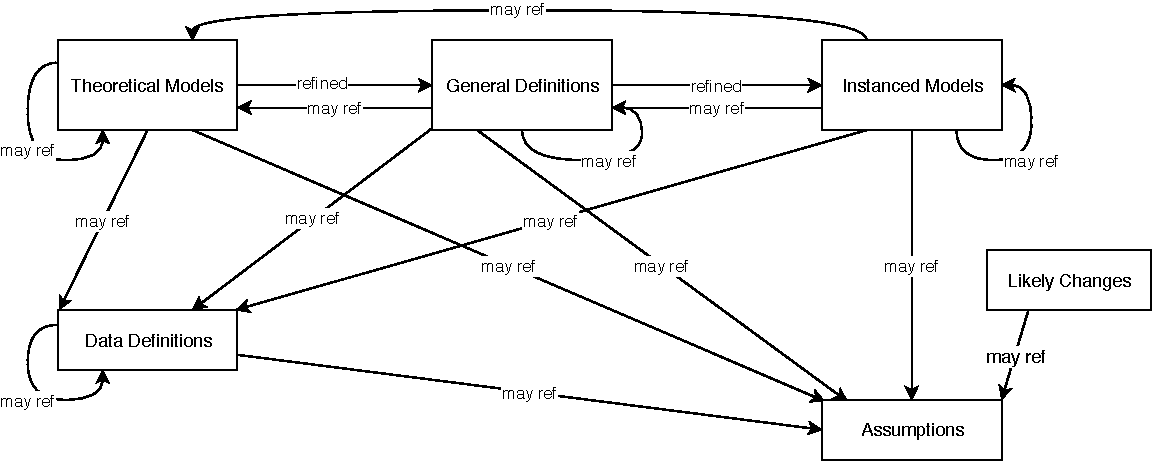
\includegraphics[scale=0.9]{figures/RelationsBetweenTM_GD_IM_DD_A.pdf}
\end{figure}

The instance models that govern \progname{} are presented in
Subsection~\ref{sec_instance}.  The information to understand the meaning of the
instance models and their derivation is also presented, so that the instance
models can be verified.

\subsubsection{Types}

\plt{This section is optional. Defining types can make the document easier to
understand.}

\subsubsection{Scope Decisions}

\plt{This section is optional.}
\subsubsection{Modelling Decisions}

\plt{This section is optional.}

\subsubsection{Assumptions} \label{sec_assumpt}

\plt{The assumptions are a refinement of the scope.  The scope is general, where
  the assumptions are specific.  All assumptions should be listed, even those
  that domain experts know so well that they are rarely (if ever) written down.}
\plt{The document should not take for granted that the reader knows which
  assumptions have been made. In the case of unusual assumptions, it is
  recommended that the documentation either include, or point to, an explanation
  and justification for the assumption.}
\plt{If it helps with the organization and understandability, the assumptions can be presented as sub sections.  The following sub-sections are options: background theory assumptions, helper theory assumptions, generic theory assumptions, problem specific assumptions, and rationale assumptions}

This section simplifies the original problem and helps in developing the
theoretical model by filling in the missing information for the physical system.
The numbers given in the square brackets refer to the theoretical model [TM],
general definition [GD], data definition [DD], instance model [IM], or likely
change [LC], in which the respective assumption is used.

\begin{itemize}

\item[A\refstepcounter{assumpnum}\theassumpnum \label{A_meaningfulLabel}:]
  \plt{Short description of each assumption.  Each assumption
    should have a meaningful label.  Use cross-references to identify the
    appropriate traceability to TM, GD, DD etc., using commands like dref, ddref
    etc.  Each assumption should be atomic - that is, there should not be an
    explicit (or implicit) ``and'' in the text of an assumption.}

\end{itemize}

\subsubsection{Theoretical Models}\label{sec_theoretical}

\plt{Theoretical models are sets of abstract mathematical equations or axioms
  for solving the problem described in Section ``Physical System Description''
  (Section~\ref{sec_phySystDescrip}). Examples of theoretical models are
  physical laws, constitutive equations, relevant conversion factors, etc.}

\plt{Optionally the theory section could be divided into subsections to provide more structure and improve understandability and reusability.  Potential subsections include the following: Context theories, background theories, helper theories, generic theories, problem specific theories, final theories and rationale theories.}

This section focuses on the general equations and laws that \progname{} is based
on.  \plt{Modify the examples below for your problem, and add additional models
  as appropriate.}

~\newline

\noindent
\deftheory
% #2 refname of theory
{TM:COE}
% #3 label
{Conservation of thermal energy}
% #4 equation
{
  $-{\bf \nabla \cdot q} + g$ = $\rho C \frac{\partial T}{\partial t}$
}
% #5 description
{
  The above equation gives the conservation of energy for transient heat transfer in a material
  of specific heat capacity $C$ (\si{\joule\per\kilogram\per\celsius}) and density $\rho$ 
  (\si{\kilogram\per\cubic\metre}), where $\bf q$ is the thermal flux vector (\si{\watt\per\square\metre}),
  $g$ is the volumetric heat generation
  (\si{\watt\per\cubic\metre}), $T$ is the temperature
  (\si{\celsius}),  $t$ is time (\si{\second}), and $\nabla$ is
  the gradient operator.  For this equation to apply, other forms
  of energy, such as mechanical energy, are assumed to be negligible in the
  system (\aref{A_OnlyThermalEnergy}).  In general, the material properties ($\rho$ and $C$) depend on temperature.
}
% #6 Notes
{
None.
}
% #7 Source
{
  \url{http://www.efunda.com/formulae/heat_transfer/conduction/overview_cond.cfm}
}
% #8 Referenced by
{
  \dref{ROCT}
}
% #9 Preconditions
{
None
}
% #1 derivation - not applicable by default
{}

\plt{``Ref.\ By'' is used repeatedly with the different types of information.
  This stands for Referenced By.  It means that the models, definitions and
  assumptions listed reference the current model, definition or assumption.
  This information is given for traceability.  Ref. By provides a pointer in the
  opposite direction to what we commonly do.  You still need to have a reference
  in the other direction pointing to the current model, definition or
  assumption.  As an example, if TM1 is referenced by GD2, that means that GD2 will
  explicitly include a reference to TM1.}

~\newline

\subsubsection{General Definitions}\label{sec_gendef}

\plt{General Definitions (GDs) are a refinement of one or more TMs, and/or of
  other GDs.  The GDs are less abstract than the TMs.  Generally the reduction
  in abstraction is possible through invoking (using/referencing) Assumptions.
  For instance, the TM could be Newton's Law of Cooling stated abstracting.  The
  GD could take the general law and apply it to get a 1D equation.}

This section collects the laws and equations that will be used in building the
instance models.

\plt{Some projects may not have any content for this section, but the section
  heading should be kept.}  \plt{Modify the examples below for your problem, and
  add additional definitions as appropriate.}

~\newline

\noindent
\begin{minipage}{\textwidth}
\renewcommand*{\arraystretch}{1.5}
\begin{tabular}{| p{\colAwidth} | p{\colBwidth}|}
\hline
\rowcolor[gray]{0.9}
Number& GD\refstepcounter{defnum}\thedefnum \label{NL}\\
\hline
Label &\bf Newton's law of cooling \\
\hline
% Units&$MLt^{-3}T^0$\\
% \hline
SI Units&\si{\watt\per\square\metre}\\
\hline
Equation&$ q(t) = h \Delta T(t)$  \\
\hline
Description &
Newton's law of cooling describes convective cooling from a surface.  The law is
stated as: the rate of heat loss from a body is proportional to the difference
in temperatures between the body and its surroundings.
\\
& $q(t)$ is the thermal flux (\si{\watt\per\square\metre}).\\
& $h$ is the heat transfer coefficient, assumed independent of $T$ (\aref{A_hcoeff})
	(\si{\watt\per\square\metre\per\celsius}).\\
&$\Delta T(t)$= $T(t) - T_{\text{env}}(t)$ is the time-dependent thermal gradient
between the environment and the object (\si{\celsius}).
\\
\hline
  Source & Citation here \\
  \hline
  Ref.\ By & \ddref{FluxCoil}, \ddref{FluxPCM}\\
  \hline
\end{tabular}
\end{minipage}\\

\subsubsection*{Detailed derivation of simplified rate of change of temperature}

\plt{This may be necessary when the necessary information does not fit in the
  description field.}
\plt{Derivations are important for justifying a given GD.  You want it to be
  clear where the equation came from.}

\subsubsection{Data Definitions}\label{sec_datadef}

\plt{The Data Definitions are definitions of symbols and equations that are
  given for the problem.  They are not derived; they are simply used by other
  models.  For instance, if a problem depends on density, there may be a data
  definition for the equation defining density.  The DDs are given information
  that you can use in your other modules.}

\plt{All Data Definitions should be used (referenced) by at least one other
  model.}

This section collects and defines all the data needed to build the instance
models. The dimension of each quantity is also given.  \plt{Modify the examples
  below for your problem, and add additional definitions as appropriate.}

~\newline

\noindent
\begin{minipage}{\textwidth}
\renewcommand*{\arraystretch}{1.5}
\begin{tabular}{| p{\colAwidth} | p{\colBwidth}|}
\hline
\rowcolor[gray]{0.9}
Number& DD\refstepcounter{datadefnum}\thedatadefnum \label{FluxCoil}\\
\hline
Label& \bf Heat flux out of coil\\
\hline
Symbol &$q_C$\\
\hline
% Units& $Mt^{-3}$\\
% \hline
  SI Units & \si{\watt\per\square\metre}\\
  \hline
  Equation&$q_C(t) = h_C (T_C - T_W(t))$, over area $A_C$\\
  \hline
  Description & 
                $T_C$ is the temperature of the coil (\si{\celsius}).  $T_W$ is the temperature of the water (\si{\celsius}).  
                The heat flux out of the coil, $q_C$ (\si{\watt\per\square\metre}), is found by
                assuming that Newton's Law 
                of Cooling applies (\aref{A_Newt_coil}).  This law (\dref{NL}) is used on the surface of
                the coil, which has area $A_C$ (\si{\square\metre}) and heat 
                transfer coefficient $h_C$
                (\si{\watt\per\square\metre\per\celsius}).  This equation
                assumes that the temperature of the coil is constant over time (\aref{A_tcoil}) and that it does not vary along the length
                of the coil (\aref{A_tlcoil}).
  \\
  \hline
  Sources& Citation here \\
  \hline
  Ref.\ By & \iref{ewat}\\
  \hline
\end{tabular}
\end{minipage}\\

\subsubsection{Data Types}\label{sec_datatypes}

\plt{This section is optional.  In many scientific computing programs it isn't
  necessary, since the inputs and outpus are straightforward types, like reals,
  integers, and sequences of reals and integers.  However, for some problems it
  is very helpful to capture the type information.}

\plt{The data types are not derived; they are simply stated and used by other
  models.}

\plt{All data types must be used by at least one of the models.}

\plt{For the mathematical notation for expressing types, the recommendation is
  to use the notation of~\citet{HoffmanAndStrooper1995}.}

This section collects and defines all the data types needed to document the
models. \plt{Modify the examples below for your problem, and add additional
  definitions as appropriate.}

~\newline

\noindent
\begin{minipage}{\textwidth}
\renewcommand*{\arraystretch}{1.5}
\begin{tabular}{| p{\colAwidth} | p{\colBwidth}|}
  \hline
  \rowcolor[gray]{0.9}
  Type Name & Name for Type\\
  \hline
  Type Def & mathematical definition of the type\\
  \hline
  Description & description here
  \\
  \hline
  Sources & Citation here, if the type is borrowed from another source\\
  \hline
\end{tabular}
\end{minipage}\\

\subsubsection{Instance Models} \label{sec_instance}    

\plt{The motivation for this section is to reduce the problem defined in
  ``Physical System Description'' (Section~\ref{sec_phySystDescrip}) to one
  expressed in mathematical terms. The IMs are built by refining the TMs and/or
  GDs.  This section should remain abstract.  The SRS should specify the
  requirements without considering the implementation.}

This section transforms the problem defined in Section~\ref{Sec_pd} into 
one which is expressed in mathematical terms. It uses concrete symbols defined 
in Section~\ref{sec_datadef} to replace the abstract symbols in the models 
identified in Sections~\ref{sec_theoretical} and~\ref{sec_gendef}.

The goals \plt{reference your goals} are solved by \plt{reference your instance
  models}.  \plt{other details, with cross-references where appropriate.}
\plt{Modify the examples below for your problem, and add additional models as
  appropriate.}

~\newline

%Instance Model 1

\noindent
\begin{minipage}{\textwidth}
\renewcommand*{\arraystretch}{1.5}
\begin{tabular}{| p{\colAwidth} | p{\colBwidth}|}
  \hline
  \rowcolor[gray]{0.9}
  Number& IM\refstepcounter{instnum}\theinstnum \label{ewat}\\
  \hline
  Label& \bf Energy balance on water to find $T_W$\\
  \hline
  Input&$m_W$, $C_W$, $h_C$, $A_C$, $h_P$, $A_P$, $t_\text{final}$, $T_C$, 
  $T_\text{init}$, $T_P(t)$ from \iref{epcm}\\
  & The input is constrained so that $T_\text{init} \leq T_C$ (\aref{A_charge})\\
  \hline
  Output&$T_W(t)$, $0\leq t \leq t_\text{final}$, such that\\
  &$\frac{dT_W}{dt} = \frac{1}{\tau_W}[(T_C - T_W(t)) + {\eta}(T_P(t) - T_W(t))]$,\\
  &$T_W(0) = T_P(0) = T_\text{init}$ (\aref{A_InitTemp}) and $T_P(t)$ from \iref{epcm} \\
  \hline
  Description&$T_W$ is the water temperature (\si{\celsius}).\\
  &$T_P$ is the PCM temperature (\si{\celsius}).\\
  &$T_C$ is the coil temperature (\si{\celsius}).\\
  &$\tau_W = \frac{m_W C_W}{h_C A_C}$ is a constant (\si{\second}).\\
  &$\eta = \frac{h_P A_P}{h_C A_C}$ is a constant (dimensionless).\\
  & The above equation applies as long as the water is in liquid form,
  $0<T_W<100^o\text{C}$, where $0^o\text{C}$ and $100^o\text{C}$ are the melting
  and boiling points of water, respectively (\aref{A_OpRange}, \aref{A_Pressure}).
  \\
  \hline
  Sources& Citation here \\
  \hline
  Ref.\ By & \iref{epcm}\\
  \hline
\end{tabular}
\end{minipage}\\

%~\newline

\subsubsection*{Derivation of ...}

\plt{The derivation shows how the IM is derived from the TMs/GDs.  In cases
  where the derivation cannot be described under the Description field, it will
  be necessary to include this subsection.}

\subsubsection{Input Data Constraints} \label{sec_DataConstraints}    

Table~\ref{TblInputVar} shows the data constraints on the input output
variables.  The column for physical constraints gives the physical limitations
on the range of values that can be taken by the variable.  The column for
software constraints restricts the range of inputs to reasonable values.  The
software constraints will be helpful in the design stage for picking suitable
algorithms.  The constraints are conservative, to give the user of the model the
flexibility to experiment with unusual situations.  The column of typical values
is intended to provide a feel for a common scenario.  The uncertainty column
provides an estimate of the confidence with which the physical quantities can be
measured.  This information would be part of the input if one were performing an
uncertainty quantification exercise.

The specification parameters in Table~\ref{TblInputVar} are listed in
Table~\ref{TblSpecParams}.

\begin{table}[!h]
  \caption{Input Variables} \label{TblInputVar}
  \renewcommand{\arraystretch}{1.2}
\noindent \begin{longtable*}{l l l l c} 
  \toprule
  \textbf{Var} & \textbf{Physical Constraints} & \textbf{Software Constraints} &
                             \textbf{Typical Value} & \textbf{Uncertainty}\\
  \midrule 
  $L$ & $L > 0$ & $L_{\text{min}} \leq L \leq L_{\text{max}}$ & 1.5 \si[per-mode=symbol] {\metre} & 10\%
  \\
  \bottomrule
\end{longtable*}
\end{table}

\noindent 
\begin{description}
\item[(*)] \plt{you might need to add some notes or clarifications}
\end{description}

\begin{table}[!h]
\caption{Specification Parameter Values} \label{TblSpecParams}
\renewcommand{\arraystretch}{1.2}
\noindent \begin{longtable*}{l l} 
  \toprule
  \textbf{Var} & \textbf{Value} \\
  \midrule 
  $L_\text{min}$ & 0.1 \si{\metre}\\
  \bottomrule
\end{longtable*}
\end{table}

\subsubsection{Properties of a Correct Solution} \label{sec_CorrectSolution}

\noindent
A correct solution must exhibit \plt{fill in the details}.  \plt{These
  properties are in addition to the stated requirements.  There is no need to
  repeat the requirements here.  These additional properties may not exist for
  every problem.  Examples include conservation laws (like conservation of
  energy or mass) and known constraints on outputs, which are usually summarized
  in tabular form.  A sample table is shown in Table~\ref{TblOutputVar}}

\begin{table}[!h]
\caption{Output Variables} \label{TblOutputVar}
\renewcommand{\arraystretch}{1.2}
\noindent \begin{longtable*}{l l} 
  \toprule
  \textbf{Var} & \textbf{Physical Constraints} \\
  \midrule 
  $T_W$ & $T_\text{init} \leq T_W \leq T_C$ (by~\aref{A_charge})
  \\
  \bottomrule
\end{longtable*}
\end{table}

\plt{This section is not for test cases or techniques for verification and
  validation.  Those topics will be addressed in the Verification and Validation
  plan.}

\fi

% section (new) 5: Stakeholders
\section{Stakeholders}

The stakeholders for this game project are those with vested interests in its development, release, and continued use. While there may be individuals with vested interest in \textit{Dice Duels: Duel of the Eights}, they all fall within the broader categories below and generally act as a member of the whole rather than an individual stakeholder. Stakeholders for the capstone but not for the project itself are included in some sections below, but are not considered a stakeholder of the project due to not influencing the direction and development of the game outside of requiring a certain challenge level and documentation.

\subsection{Traditional Yahtzee enthusiasts}

\begin{itemize}
	\item \textbf{Demographics:} Generally older players who have nostalgia for the classic Yahtzee game. They may have experience with the physical dice game playing with family and friends and seek a familiar experience to bring back memories and connect with people. 
	\item \textbf{Technical Comfort Level:} May be lacking in experience with technology and be more comfortable with straightforward,  user-friendly interfaces and are likely to appreciated clear instructions.
	\item \textbf{Motivations:}
	\begin{itemize}
		\item \textit{Nostalgia.} They seek to relive the classic Yahtzee experience in a more accessible format.
		\item \textit{Social connection.} They are interested in playing with friends they may not be able to meet in person.
		\item \textit{Relaxed gameplay.} They generally prefer low-stakes slower-paced gameplay that doesn't require complex strategies or fast decision making. They are more likely to appreciate a more relaxed experience.
	\end{itemize}
	\item \textbf{Preferences:}
	\begin{itemize}
		\item \textit{Classic game mode.} They'll likely be drawn to a game mode that replicates the original Yahtzee experience.
		\item \textit{Simplicity over customization.} While they may be willing to try out some customization, they may prefer options that don't stray too far from the classic.
		\item \textit{Minimalistic design.} An interface that's easy on the eyes with intuitive navigation will help make the experience enjoyable for them.
	\end{itemize}
\end{itemize}

\subsection{Video Game enthusiasts}

\begin{itemize}
	\item \textbf{Demographics:} A diverse group spanning casual players to more experienced players focused on optimization, they are familiar with online multiplayer games and are comfortable with technology and video games.
	\item \textbf{Technical Comfort Level:} Most typical gamers are comfortable with technology, online multiplayer, and faster-paced games. They enjoy exploring game mechanics and may be open to more complex overlapping game mechanics. Are comfortable downloading a new video game with straightforward procedures.
	\item \textbf{Motivation:}
	\begin{itemize}
		\item \textit{Challenge and skill expression.} They're interested in games that allow for strategy and competitive play where skill and quick decision-making have an impact on the outcome.
		\item \textit{Engagement.} Video game enthusiasts seek a fast-paced experience with more action and reward cycles that provide instant feedback and keep them engaged.
		\item \textit{Replayability.} They generally enjoy experiences with unique challenges every time they play and can develop strategies over multiple runs.
	\end{itemize}
	\item \textbf{Preferences:}
	\begin{itemize}
		\item \textit{Customization and variability.} They are likely to appreciate the ability to customize gameplay to explore possibilities and develop a game system that is challenging but enjoyable for them.
		\item \textit{Faster game modes.} They may enjoy options that speed up gameplay, such as round timers or different scoring methods that add intensity and variety.
		\item \textit{Reactive feedback.} Faster-paced action and instant feedback to keep them engaged would be preferred over slower gameplay.
	\end{itemize}
\end{itemize}

\subsection{Personas}

\begin{itemize}
	\item \textbf{Joan, 55 years old (The Nostalgic Yahtzee Player)} Joan enjoys simple board games that remind her of family gatherings. She values a straightforward interface, classic gameplay, and the option to play casually with friends over the internet when they cannot meet in person.
	\item \textbf{James, 24 years old (The Casual Gamer)} James plays games on the weekends with friends. He enjoys the flexibility of customizable game modes and fast-paced rounds. Alex values multiplayer gameplay with friends and occasional solo play.
	\item \textbf{Julian, 19 years old (The Competitive Gamer)} Julian enjoys strategic games that involve skill, competition, and learning over time. He prefers playing with friends that are similarly competitive, customization options, and post-game statistics to analyze his performance.
\end{itemize}

\subsection{Priorities Assigned to Users}

\begin{itemize}
	\item \textbf{Primary Priority:} Casual and competitive video game enthusiasts would be the primary priority as they are the most plentiful and would be most likely to come across the game to play it. There is currently no game that provides customizable Yahtzee-like mechanics, and with feedback and testing, the game can be made to tailor to their preferences and be engaging.
	\item \textbf{Secondary Priority:} Traditional Yahtzee enthusiasts are a secondary priority in that using customization mechanics their preferred classic game can be recreated, but the game system overall would be more than just that. Their needs for a simple and intuitive user interface must be taken into consideration, as must options be available for their experience to likewise be enjoyable.
	\item \textbf{Tertiary Priority:} Outside of the context of stakeholders for the program, there are stakeholders for the capstone project. Their considerations do not shape the game itself as they are unlikely to play the game, but rather require a specific challenge level and documentation to be produced. As such, they can be considered tertiary despite not being stakeholders to the game unless also included in one of the above stakeholder groups.
\end{itemize}

\subsection{User Participation}

\begin{itemize}
	\item \textbf{Development Phase:} Selected playtesters and the development team will regularly engage with the game throughout the development cycle to identify bugs and shape the user experience.
	\item \textbf{Testing Phase:} Both playtesters and target user groups will participate in beta testing to validate usability, customization options, and multiplayer functionality.
	\item \textbf{Feedback Phase:} In the feedback phase, when functionality is mostly validated, users will provide feedback through surveys and interviews to refine the game before a final release.
\end{itemize}

\subsection{Ongoing Support}

This project will be released with a final build that is complete and of quality. Since this game will also be released under a permissive license, the codebase will be publicly available on GitHub, allowing others to further develop it and add features they themselves may wish to have available, or fix any bugs that may be present. The current developers may also be available in their free time if this project or a spin-off is something that will continue past the capstone project timeframe.


% section 6: Requirements
% section 7: Requirements Implementatino Roadmap
\section{Requirements}

\subsection{Functional Requirements}

\begin{enumerate}[label=R\arabic*, start=1, left=0pt]

    \item \label{R1} The game shall support an online player vs player mode, where 2 players can play against each other.
    \begin{description}
        \item[Rationale:] Player vs player support is a central functionality for this game and one that enhances the overall enjoyment of the game by fostering a more social game dynamic.
    \end{description}

    \item \label{R2} The game shall handle score calculations using similar rules to standard Yahtzee under default game settings.
    \begin{description}
        \item[Rationale:] Score calculations that follow from a well established, and well balanced game will help users jump into the game faster and foster a more fair game experience.
    \end{description}

    \item \label{R3} The game shall simulate realistic physics for 3D dice rolls with true randomness on every roll that replicates accurately to all users.
    \begin{description}
        \item[Rationale:] It is important that players get to visually see the dice roll and feel that the outcome of the roll is not clearly predetermined in order to enhance the user experience and maintain continuity between the game and real life.
    \end{description}

    \item \label{R4} The game shall use the real outcome of a roll to get the values from the dice.
    \begin{description}
        \item[Rationale:] In order to get true randomness off a simulated dice roll, it makes the most sense to actually just simulate the roll and read the result rather than precalculating the results and forcing the roll to match the output.
    \end{description}

    \item \label{R5} The game shall support both regular six-sided dice and a set of dice with different number of sides, such as octahedral dice.
    \begin{description}
        \item[Rationale:] By providing support for more dice types, we can increase the level of complexity of the game for users that are looking for a more interesting variation of the game.
    \end{description}

    \item \label{R6} The game shall implement a simultaneous turn based mechanism such that each player (or computer) takes a turn at the same time and then results are revealed simultaneously to each other at each dice roll.
    \begin{description}
        \item[Rationale:] This allows users to play together syncronously, while preserving the secrecy of each dice roll so that no player gets an advantage by knowing whether their opponent has rolled well or not.
    \end{description}

    \item \label{R7} The game shall allow players to pick which dice they would like to use for each roll, and which dice they would like to omit.
    \begin{description}
        \item[Rationale:] This is an important part of standard game rules, and also increases the range of strategic decision making that players get to have.
    \end{description}

    \item \label{R8} The game shall display some sort of user interface to display scores, number of rolls, time limits, state of dice, and player names.
    \begin{description}
        \item[Rationale:] Some form of user interface is necessary to convey important game information to the player.
    \end{description}

    \item \label{R9} The game shall provide controls for the player to modify the game settings to access unique variants of the game.
    \begin{description}
        \item[Rationale:] A core part of our team's vision for this game is that players should be able to customize their playing experience by altering things like; number of dice, type of dice used, time settings, and scoring methods.
    \end{description}

    \item \label{R10} The game shall provide presets for different game modes.
    \begin{description}
        \item[Rationale:] This should help new players get used to the game before exploring more unique setting configurations.
    \end{description}

%   REQUIREMENTS RELATING TO STRETCH GOALS LISTED BELOW:::::::
    \textit{**** The following requirements relate to our stretch goals ****}
    \item \label{R11} The game shall support a local player vs player mode, where 2 players can play against each other on the same computer.
    \begin{description}
        \item[Rationale:] Given that this is a turn based game it is perfectly possible for this game to be setup with 2 player functionality on one device. This simply increases the number of ways in which the game can be played.
    \end{description}

    \item \label{R12} The game shall support a player vs computer mode, where 1 player can play against another entity without needing to find a human match.
    \begin{description}
        \item[Rationale:] Player vs computer support is important for instances where a user may not be able to find a human match to play against.
    \end{description}

    \item \label{R13} The game shall implement some sort of algorithmic computer opponent for  player vs computer gameplay option.
    \begin{description}
        \item[Rationale:] For player vs computer to function, some sort of algorithmic opponent will be necessary to implement the computer player or else there will be no challenge for the human player.
    \end{description}

    \item \label{R14} The game shall implement online matchmaking.
    \begin{description}
        \item[Rationale:] For players that want to play the game against a real opponent but don't know anyone who is available to play against them, this is a great way for that player to find someone to play against.
    \end{description}

    \item \label{R15} The game shall provide the option to save specific game settings to be reused in future sessions.
    \begin{description}
        \item[Rationale:] For frequent players of the game, they may have a preferred custom variation of the game settings that they may wish to save rather than having to input the game settings on every new game.
    \end{description}

    \item \label{R16} The game shall display round statistics to each player at the end of every round.
    \begin{description}
        \item[Rationale:] Players will likely want to see some statistics at the end of the round to quantify how well they played.
    \end{description}

%   REQUIREMENTS ADDED DUE TO HAZARD ANALYSIS LISTED BELOW:::::::
    \textit{**** The following requirements relate to our hazard analysis ****}
    \item \label{R17} The game shall always show the correct current state accurately.
    \begin{description}
        \item[Rationale:] The player needs to be able to understand the current state of the game to understand their current standings, and strategic the next move. Similarly, the current state indicates what is the next action to be done by the user. This is extended to states outside of an active game such as game settings selection, match-up, and system settings selection.
    \end{description}

\end{enumerate}

\subsection{Non-Functional Requirements}

\begin{enumerate}[label=NFR\arabic*, start=1, left=0pt]

    \item \label{NFR1} \textbf{Performance} The game shall maintain a frame rate of at least 30 FPS at all times.
    \begin{description}
        \item[Rationale:] Players need the frame rate of the game to be high enough at all times to see what’s going on.
    \end{description}

    \item \label{NFR2} \textbf{Usability} The game shall implement a clear and easy to use/understand user interface.
    \begin{description}
        \item[Rationale:] Users should not struggle to figure out where controls are or how certain features work. This would create a barrier to entry for new players, and it would be best if players could pick up this game and its controls with little difficulty or time required.
    \end{description}

    \item \label{NFR3} \textbf{Portability} The game shall be supported on systems running Windows 10 or later.
    \begin{description}
        \item[Rationale:] Most PC users use Windows 10 or 11, so ensuring that the game ports well to these operating systems is an important requirement if we want to reach a large demographic of users.
    \end{description}

    \item \label{NFR4} \textbf{Reliability} Multiplayer games of Yahtzee should crash less than 1\% of the time.
    \begin{description}
        \item[Rationale:] Players need to feel that the game is reliable and should not need to be concerned about the game crashing in the middle of a round.
    \end{description}

    \item \label{NFR5} \textbf{Responsiveness} The game shall respond to inputs from the user within 500 milliseconds in the worst case.
    \begin{description}
        \item[Rationale:] This figure represents a minimum acceptable response. If a user needs to wait longer than this to see the result of their input, they may become frustrated and even try spamming the control.
    \end{description}

    \item \label{NFR6} \textbf{Modularity} The game’s codebase shall be modular, such that it is easily extendable and reusable, and allows for quick fixes to bugs that may occur.
    \begin{description}
        \item[Rationale:] Our team has minimum goals in mind for what this game must be upon release, but to be able to continue updating the game to meet stretch goals, our codebase should be designed with modularity in mind to streamline the development process.
    \end{description}

    \item \label{NFR7} \textbf{Efficiency} The game shall be optimized to run on lower end systems which might have minimal CPU and GPU resources.
    \begin{description}
        \item[Rationale:] The game that our team is developing is not such a graphically or computationally intensive game that it should require high-end PCs to run. Additionally, being able to run the game on lower-end systems will allow our game to reach a broader audience.
    \end{description}

    \item \label{NFR8} \textbf{Enjoyability} The game shall be found enjoyable by at least 75\% of users.
    \begin{description}
        \item[Rationale:] The game should appeal to the majority of its users, because if it doesn't then the game serves no particular purpose.
    \end{description}

    \item \label{NFR9} \textbf{Appearance} The game shall maintain a consistent UI style and 3D visual style throughout all in game views.
    \begin{description}
        \item[Rationale:] A style that evokes some sense of continuity throughout the game is important to help users get used to the layout faster and to give the appearance of a more professionally developed gaming experience.
    \end{description}

%   REQUIREMENTS RELATING TO STRETCH GOALS LISTED BELOW:::::::
    \textit{**** The following requirements relate to our stretch goals ****}
    \item \label{NFR10} \textbf{Portability} The game shall be supported on MacOS devices.
    \begin{description}
        \item[Rationale:] There are many users who use MacOS devices and would be a good target audience for this game.
    \end{description}

\end{enumerate}

\section{Requirements Implementation Roadmap (Phase In Plan)}

The implementation roadmap outlines the priority and timeline for completing each functional and non-functional requirement for the game. Requirements are categorized into four main priority sections to ensure a clear implementation plan throughout development.

\subsection{Critical Priority}
These functional and non-functional requirements are necessary for every stable build generated and are required through all stages of development, hence have no specific Phase In plan date.
\begin{itemize}
    \item \textbf{R2:} The game must allow players to roll up to five dice simultaneously.
    \item \textbf{R3:} Players must be able to re-roll selected dice up to two times per turn.
    \item \textbf{R4:} The game must implement scoring categories, such as "Three of a Kind," "Four of a Kind," and "Full House."
    \item \textbf{R5:} The game must support calculating and displaying the current score for each player.
    \item \textbf{R8:} The game must provide a user interface for players to select scoring categories and view scores.
    \item \textbf{R17:} The game must support networked multiplayer functionality for PvP matches.
\end{itemize}

\subsection{High Priority}
These requirements are required for all stable builds but are flexible based on the specific game variant implementation, hence have no specific Phase In plan date.
\begin{itemize}
    \item \textbf{R1:} The game must provide a digital representation of a Yahtzee scorecard.
    \item \textbf{R6:} Players must be able to end their turn, and scores must be locked in accordingly.
    \item \textbf{R7:} The game must display the current round number and the total number of rounds.
    \item \textbf{R9:} The game must include audio cues for rolling dice and scoring actions.
    \item \textbf{R10:} The game must include visual effects to enhance the player experience, such as dice animations.
\end{itemize}

\subsection{Non-Functional Requirements Priority}
These non-functional requirements (NFRs) are Medium Priority and will be improved upon during the course of development, starting with lower standards of NFR satisfaction, with the goal of satisfying each NFR completely by Final Demo.
\begin{itemize}
    \item \textbf{NFR1:} The game should have an average response time of less than 100 ms for player interactions.
    \item \textbf{NFR2:} The game should provide a consistent frame rate of at least 30 FPS.
    \item \textbf{NFR3:} The game should support a variety of screen resolutions and aspect ratios.
    \item \textbf{NFR4:} The game must handle network disconnections gracefully, allowing players to reconnect.
    \item \textbf{NFR5:} The game should provide accessibility features, such as colorblind-friendly UI options.
    \item \textbf{NFR6:} The game should support cross-platform play between different operating systems.
    \item \textbf{NFR7:} The game should ensure data privacy and protection, including encryption of sensitive player data.
    \item \textbf{NFR8:} The game should include an in-game tutorial to guide new players.
    \item \textbf{NFR9:} The game should have logging and diagnostics features for debugging purposes.
\end{itemize}

\subsection{Stretch Goals}
Lower Priority, and will be tackled in order of individual priority, in the given order, based on scope during or at the end of the project, or post capstone.
\begin{itemize}
    \item \textbf{R15:} The game should include leaderboards to track high scores across all players.
    \item \textbf{R16:} The game should allow players to customize their dice and scorecard appearance.
    \item \textbf{R14:} The game should support in-game chat for players during multiplayer matches.
    \item \textbf{R11:} The game should include soundtracks that can be toggled by players.
    \item \textbf{NFR10:} The game should support integration with third-party social media for sharing scores.
    \item \textbf{R12:} The game should include a feature to save and resume matches.
    \item \textbf{R13:} The game should support various game modes, such as "Classic Yahtzee" and "Custom Rules."
\end{itemize}




% section 8: Standards
% section 9: Compliance Roadmap
\newpage
\section{Standards, Codes, Legal, and Regulatory Factors}    

Developing an online multiplayer game requires adherence to various standards, codes, legal, and regulatory factors to ensure a safe, fair, and compliant gaming experience. The following standards are identified for the multiplayer aspect of the game, especially in the context of player-versus-player (PvP) matches:

\subsection{Data Privacy and Protection}
\begin{itemize}
    \item \textbf{GDPR (General Data Protection Regulation)}: Given that the game may involve players from the European Union, compliance with GDPR is essential. This includes ensuring user consent for data collection, providing clear privacy policies, and safeguarding player data.
    \item \textbf{CCPA (California Consumer Privacy Act)}: If players are based in California, the game must comply with CCPA to give users control over their personal information.
    \item \textbf{COPPA (Children's Online Privacy Protection Act)}: If the game targets children under 13, compliance with COPPA is mandatory to protect children’s privacy.
\end{itemize}

\subsection{Network and Online Standards}
\begin{itemize}
    \item \textbf{IEEE 802.11 (Wi-Fi Standards)}: Ensuring reliable local area network (LAN) connectivity follows IEEE 802.11 standards to provide consistent communication quality.
    \item \textbf{WebSockets (RFC 6455)}: The use of WebSockets for real-time communication between players must comply with RFC 6455 to ensure reliable, secure data exchange.
\end{itemize}

\subsection{Game Fairness and Anti-Cheating Measures}
\begin{itemize}
    \item \textbf{ISO/IEC 27001 (Information Security Management)}: Implementing practices from ISO/IEC 27001 helps in managing game security, reducing the risk of cheating, and protecting the game from malicious activities.
    \item \textbf{Fair Play Guidelines}: To ensure fair play in PvP matches, the game should adopt fair matchmaking and anti-cheating measures, such as monitoring unusual behavior and implementing server-side verification of actions.
\end{itemize}

\subsection{Legal Considerations for Online Play}
\begin{itemize}
    \item \textbf{Terms of Service and End-User License Agreement (EULA)}: A clear EULA must be provided, detailing acceptable behavior, limitations of liability, and consequences for misuse or cheating.
    \item \textbf{Content Rating Standards}: The game must be rated appropriately, such as following the \textbf{ESRB (Entertainment Software Rating Board)} or \textbf{PEGI (Pan European Game Information)} standards, to ensure suitability for the intended audience.
\end{itemize}

\subsection{Accessibility Standards}
\begin{itemize}
    \item \textbf{WCAG (Web Content Accessibility Guidelines) 2.1}: For an inclusive experience, the game’s online features and user interface should follow WCAG 2.1 guidelines, ensuring accessibility for players with disabilities.
\end{itemize}

\subsection{Intellectual Property and Copyright}
\begin{itemize}
    \item \textbf{Copyright Compliance}: The game must avoid unauthorized use of copyrighted material, including sound effects, graphics, and other assets. Original content must be used, or appropriate licenses must be obtained.
    \item \textbf{Trademark Considerations}: Any use of trademarks must be properly authorized to avoid infringement issues.
\end{itemize}

\subsection{Regulatory Requirements for Online Play}
\begin{itemize}
    \item \textbf{Online Gambling Regulations}: If any aspect of the game involves virtual currency or random rewards, it may fall under online gambling regulations in certain jurisdictions. The game must be reviewed for compliance with applicable laws to avoid any unintended legal issues.
    \item \textbf{Consumer Protection Laws}: Compliance with consumer protection laws is crucial, ensuring transparency in in-game purchases and providing users with refund policies.
\end{itemize}

By adhering to these standards, codes, and legal factors, the development of the online multiplayer game will ensure a fair, compliant, and enjoyable experience for all players, while minimizing legal and regulatory risks.

\newpage
\section{Standards Compliance Roadmap}

The following compliance roadmap outlines when each of the identified standards will be adhered to during the development of the online multiplayer game:

\begin{itemize}
\item \textbf{Data Privacy and Protection (GDPR, CCPA, COPPA)}: Compliance will be met by the Final Demo.
\item \textbf{Network and Online Standards (IEEE 802.11)}: Compliance will be met by the Final Demo.
\item \textbf{Network and Online Standards (WebSockets)}: Compliance will be addressed post-capstone based on the game's scale.
\item \textbf{Game Fairness and Anti-Cheating Measures (ISO/IEC 27001)}: Compliance will be addressed post-capstone based on the game's scale.
\item \textbf{Game Fairness and Anti-Cheating Measures (Fair Play Guidelines)}: Compliance will be met by the Final Demo.
\item \textbf{Legal Considerations for Online Play (Terms of Service, EULA, Content Rating Standards)}: Compliance will be met by the Final Demo.
\item \textbf{Accessibility Standards (WCAG 2.1)}: Compliance will be addressed post-capstone based on the game's scale.
\item \textbf{Intellectual Property and Copyright (Copyright Compliance, Trademark Considerations)}: Compliance will be continuously verified, with final verification by the Final Demo.
\item \textbf{Regulatory Requirements for Online Play (Online Gambling Regulations)}: Compliance may be required post-capstone based on the direction of the game and will be evaluated accordingly.
\item \textbf{Regulatory Requirements for Online Play (Consumer Protection Laws)}: Compliance will be met by the Final Demo if the game direction leads to the introduction of in-game purchases.
\end{itemize}

% section 10: Likely Changes
% section 11: Unlikely Changes
\section{Likely Changes}    

\noindent \begin{itemize}

\item[LC\refstepcounter{lcnum}\thelcnum\label{LC_meaningfulLabel}:] Add other non-dice based probabilities (cards,etc)

\begin{itemize}
	\item If the scope of our game permits an addition, we may consider adding non-dice based probabilities into our games, such as playing cards, in order to provide more variety for the user.
\end{itemize}

\item[LC\refstepcounter{lcnum}\thelcnum\label{LC_meaningfulLabel}:] the amount and variability of dice options may increase and decrease based on the scope of the project

\begin{itemize}
	\item As the Scope of our project increase and decreases, we will consider experimenting with different amounts and types of dice. and should circumstances allow, we may choose to add or remove these different options for our game.
\end{itemize}

\item[LC\refstepcounter{lcnum}\thelcnum\label{LC_meaningfulLabel}:] We may expand comparability to other operating systems depending of the scope of the project (Mac OS, etc).

\begin{itemize}
	\item While we will initially design our system to work on Windows 10/11 devices, should the scope of our project expand, we are likely to adapt our system to work on other OS systems too such as Mac OS, or Linux, allowing our product to reach more players.
\end{itemize}

\item[LC\refstepcounter{lcnum}\thelcnum\label{LC_meaningfulLabel}:] We may change how the scores are calculated.

\begin{itemize}
	\item As we change and add various options for the players, such as changing the number and types of the dice, we may need to account for the different probabilities that these new options may create, which in turn would require us to modify our scoring system to account for these radically different probabilities.
\end{itemize}

\item[LC\refstepcounter{lcnum}\thelcnum\label{LC_meaningfulLabel}:] We may expand the amount of players that can play the same game from just the initial 2 depending on scope.

\begin{itemize}
	\item While initialized for two players, it is known that Yatzee can easily support more players, given that the fundamental mechanics of the game don't change when you add them. Thus, when we stabilize our two-player multiplayer, we could expand upon it to allow more then the initial two players to play the same game, allowing more users to enjoy our product.
\end{itemize}

    


\end{itemize}

\newcounter{ucnum}

\section{Unlikely Changes}    

\noindent \begin{itemize}

\item[UC\refstepcounter{ucnum}\theucnum\label{LC_meaningfulLabel}:] We will not remove the multiplayer component of the game.

\begin{itemize}
	\item Yatzee is a social game of chance that involves chance and strategy in an appempt to get the highest score compared to other players, As such Multiplayer is a core component of the game and it must be included to ensure that an important aspect of the game isn't lost.
\end{itemize}

	
\item[UC\refstepcounter{ucnum}\theucnum\label{LC_meaningfulLabel}:] We will not remove the dice and it's probabilities 

\begin{itemize}
	\item Dice are a critical component of Yhatzee and it's variations, and the probabilities that the dices rolls provide are a core component in the way that score is calculated in game. Thus, our game will always involve the usage of dice and the calculation of the probabilities involving them.
\end{itemize}


\item[UC\refstepcounter{ucnum}\theucnum\label{LC_meaningfulLabel}:] We will not switch from our engine Godot for the duration of the project.

\begin{itemize}
	\item Godot is the engine that most of the team is familiar. Thus, it would be too risky to switch game engines and learn something the team is unfamiliar with.
\end{itemize}

\item[UC\refstepcounter{ucnum}\theucnum\label{LC_meaningfulLabel}:] We will always have customization between game variants, and not just presets.


\begin{itemize}
	\item One of the selling points for this project is to have customised settings for our game, allowing the user to tailor their experience to the way they want it. Thus, it is unlikely we will alter our plans to include this feature.
\end{itemize}

\item[LC\refstepcounter{ucnum}\theucnum\label{LC_meaningfulLabel}:] We will not change the 3D format of our game to 2D

\begin{itemize}
	\item When playing a physical game like Yahtzee, one of the most engaging aspects is the action of rolling the dice. We wish to recreate the feel of playing the physical game as closely as possible by allowing our player to be able to visually see the dice roll in a way that mirrors the physical experience.
	
	 
\end{itemize}




	


\end{itemize}

% section 12: Traceability Matrices and Graphs
\section{Traceability Matrices and Graphs}

This section has been adapted from the original "Traceability Matrices and Graphs" portion of this document, which was initially geared toward scientific computation and the dependencies between physical components. In this revised section, we focus on aligning the specific goals of the game with the corresponding requirements, design changes, and other relevant elements outlined in this document. By doing so, we aim to create a clear and structured mapping between our Goals and the necessary steps for implementation.

The traceability matrices in this section provide an overview of these connections. Where an 'X' appears in the table, it signifies that a requirement or other item was developed in response to a particular goal or is linked to that goal. Two separate tables are presented: the first traces the core Goals of the project, while the second maps the Stretch Goals, allowing for a more comprehensive understanding of how different project objectives are supported through specific requirements.

Summary definitions: (refer to Requirements section for details)
\begin{itemize}
	\item GS1: Enjoyable game
	\item GS2: Online multiplayer functionality
	\item GS3: Customizable game settings
	\item GS4: Preset game settings
	\item GS5: 3D dice rolling

	\item SG6: Local multiplayer
	\item SG7: Singleplayer variants
	\item SG8: Online matchmaking
	\item SG9: Saving custom game setting
	\item SG10: More game setting customization
	\item SG11: Visual Dice customization
	\item SG12: Post game statistics
	\item SG13: Multi-platform support
	\item SG14: Dice highlighting
\end{itemize}

\begin{table}[ht]
\centering
\begin{tabular}{|c|c|c|c|c|c|}
\hline
\textbf{Reference Item} & \textbf{GS1} & \textbf{GS2} & \textbf{GS3} & \textbf{GS4} & \textbf{GS5} \\ \hline
\textbf{R1} & &X & & & \\ \hline
\textbf{R2} & & & &X & \\ \hline
\textbf{R3} & & & & &X \\ \hline
\textbf{R4} & & & & &X \\ \hline
\textbf{R5} & & &X & & \\ \hline
\textbf{R6} & &X & & & \\ \hline
\textbf{R7} &X & & & & \\ \hline
\textbf{R8} &X & & & &X \\ \hline
\textbf{R9} & & &X & & \\ \hline
\textbf{R10} & & & &X & \\ \hline
\textbf{R17} &X & & & &X \\ \hline
\textbf{NFR1} &X & & & & \\ \hline
\textbf{NFR2} &X & & & & \\ \hline
\textbf{NFR3} & & & & & \\ \hline
\textbf{NFR4} &X & & & & \\ \hline
\textbf{NFR5} &X & & & & \\ \hline
\textbf{NFR6} & & & & & \\ \hline
\textbf{NFR7} &X & & & & \\ \hline
\textbf{NFR8} &X & & & & \\ \hline
\textbf{NFR9} &X & & & &X \\ \hline
\textbf{LC2} & & &X & & \\ \hline
\textbf{LC4} & & &X & & \\ \hline
\textbf{UC1} & &X & & & \\ \hline
\textbf{UC2} & & & & &X \\ \hline
\textbf{UC4} & & &X & & \\ \hline
\textbf{UC5} & & & & &X \\ \hline
\end{tabular}
\caption{Traceability Matrix for Goals}
\label{table:goals_traceability}
\end{table}


\begin{table}[ht]
\centering
\begin{tabular}{|c|c|c|c|c|c|c|c|c|c|}
\hline
\textbf{Reference Item} & \textbf{SG6} & \textbf{SG7} & \textbf{SG8} & \textbf{SG9} & \textbf{SG10} & \textbf{SG11} & \textbf{SG12} & \textbf{SG13} & \textbf{SG14} \\ \hline
\textbf{R11} &X & & & & & & & & \\ \hline
\textbf{R12} & &X & & & & & & & \\ \hline
\textbf{R13} & &X & & & & & & & \\ \hline
\textbf{R14} & & &X & & & & & & \\ \hline
\textbf{R15} & & & &X & & & & & \\ \hline
\textbf{R16} & & & & & & &X & & \\ \hline
\textbf{R17} & & & & & &X &X & &X \\ \hline
\textbf{NFR10} & & & & & & & &X & \\ \hline
\textbf{LC1} &X &X &X & & & & & & \\ \hline
\textbf{LC3} & & & & & & & &X & \\ \hline
\textbf{LC5} & & & & &X & & & & \\ \hline
\textbf{UC1} &X & & & & & & & & \\ \hline
\textbf{UC3} & & & & & & & &X & \\ \hline
\end{tabular}
\caption{Traceability Matrix for Stretch Goals}
\label{table:stretch_goals_traceability}
\end{table}

% section 13: Development Plan
%\section{Development Plan}

Please refer to separate development plan located in docs: \href{https://github.com/John-Popovici/duel-of-the-eights/blob/main/docs/DevelopmentPlan/DevelopmentPlan.pdf}{link}
% section added to below section for pagebreak reasons

% section 14: Values of Auxiliary Constants
\section{Values of Auxiliary Constants}

\plt{Show the values of the symbolic parameters introduced in the report.}

\plt{The definition of the requirements will likely call for SYMBOLIC\_CONSTANTS.
Their values are defined in this section for easy maintenance.}

\plt{The value of FRACTION, for the Maintainability NFR would be given here.}

% section 15: Commonailities
\section{Commonalities}

Use this section to detail the commonalities between the different games in the product family. This includes UI elements, goals, mechanics, and so on.

% section 16: Variabilities
\section{Variabilities}

This section details the variabilities between the different games in the product family, including changes in UI elements, game goals, and core mechanics.

\subsection{Number of Dice}
The number of dice used in the game can vary between different versions. Some variants may increase or decrease the number of dice to adjust the complexity and strategy of the game.

\subsection{Sides on Dice}
The number of sides on each dice can differ across game variants. This allows for customization of gameplay, where different variants may feature dice with more or fewer sides, influencing the probability and outcomes of each roll.

\subsection{Individual Sides}
The specific values or symbols on the sides of each dice can vary between versions. This variability provides an opportunity to introduce different themes or scoring dynamics depending on the game's rules.

\subsection{Scoring Calculation}
How points are calculated for different hands and the influence of dice rolls on the final score can be customized in different game variants. This allows for changes in how specific hands are valued and how scoring impacts the overall gameplay strategy.

\subsection{Time Per Turn}
The amount of time a player has to roll the dice and make their selection can be adjusted between variants. Time limits can vary, creating different levels of pressure and pacing in the game.

\subsection{Hand Restrictions}
Some game variants may restrict certain hands from being scored or may allow hands to be scored multiple times. These variations provide flexibility in game strategy and scoring dynamics.


% section 17: Values of Parameters of variations
\section{Parameters of Variations}

This section details the specific values that the variabilities between the different games in the product family can take, corresponding to the variabilities outlined in the previous section.

\subsection{Number of Dice}
The number of dice used in the game can range from 4 to 10. This allows for variations in gameplay complexity, depending on the specific variant.

\subsection{Sides on Dice}
The usable dice will be a subset of dice modeled with the following number of sides: 4, 6, 8, 10, 12. This flexibility in dice sides introduces variability in the probability and potential outcomes for each roll.

\subsection{Individual Sides}
The values displayed on the individual sides of each die can range from 1 to the respective number of sides on that die and can be displayed in different representations. This variability allows for different numerical or symbolic configurations to match specific game variants.

\subsection{Scoring Calculation}
Each hand can be assigned any integer score value or modified by factors based on the dice rolls. This provides flexibility in defining how each hand is valued in the different game variants.

\subsection{Time Per Turn}
The time allotted for each turn can range from 5 seconds to 2 minutes, or be set to unlimited. This parameter affects the pacing of the game, allowing for both fast-paced and more thoughtful gameplay.

\subsection{Hand Restrictions}
Hands can be restricted by removing up to all but one from play. Additionally, hands can be allowed to be repeated between 1 to 10 times or an unlimited number of times, giving options for different scoring strategies.



\newpage
\bibliographystyle {plainnat}
\bibliography {../../refs/References}
\newpage

% comments - to be commented out
% \noindent \plt{The following is not part of the template, just some things to consider
  when filing in the template.}

\noindent \plt{Grammar, flow and \LaTeX advice:
\begin{itemize}
\item For Mac users \texttt{*.DS\_Store} should be in \texttt{.gitignore}
\item \LaTeX{} and formatting rules
\begin{itemize}
\item Variables are italic, everything else not, includes subscripts (link to
  document)
\begin{itemize}
\item \href{https://physics.nist.gov/cuu/pdf/typefaces.pdf}{Conventions}
\item Watch out for implied multiplication
\end{itemize}
\item Use BibTeX
\item Use cross-referencing
\end{itemize}
\item Grammar and writing rules
\begin{itemize}
\item Acronyms expanded on first usage (not just in table of acronyms)
\item ``In order to'' should be ``to''
\end{itemize}
\end{itemize}}

\noindent \plt{Advice on using the template:
\begin{itemize}
\item Difference between physical and software constraints
\item Properties of a correct solution means \emph{additional} properties, not
  a restating of the requirements (may be ``not applicable'' for your problem).
  If you have a table of output constraints, then these are properties of a
  correct solution.
\item Assumptions have to be invoked somewhere
\item ``Referenced by'' implies that there is an explicit reference
\item Think of traceability matrix, list of assumption invocations and list of
  reference by fields as automatically generatable
\item If you say the format of the output (plot, table etc), then your
  requirement could be more abstract
\end{itemize}
}

% reflection
\section*{Appendix --- Reflection}

%\wss{Not required for CAS 741}

The information in this section will be used to evaluate the team members on the
graduate attribute of Lifelong Learning.  

%The purpose of reflection questions is to give you a chance to assess your own
learning and that of your group as a whole, and to find ways to improve in the
future. Reflection is an important part of the learning process.  Reflection is
also an essential component of a successful software development process.  

Reflections are most interesting and useful when they're honest, even if the
stories they tell are imperfect. You will be marked based on your depth of
thought and analysis, and not based on the content of the reflections
themselves. Thus, for full marks we encourage you to answer openly and honestly
and to avoid simply writing ``what you think the evaluator wants to hear.''

Please answer the following questions.  Some questions can be answered on the
team level, but where appropriate, each team member should write their own
response:


\begin{enumerate}
  \item What went well while writing this deliverable?
  
	\begin{itemize}
		\item The SRS document had a lot of work to be done in a lot of sections. In an effort to mitigate merge conflicts and better divide the workload, a main SRS.tex file was created which would reference and include other .tex files which contain the information for the sections. - John P.
		\item All team members were able to contribute to the document. Sections were divided up well so that each team member could focus on their own specific part. - Isaac G.
    \item Team members communicated often and effectively. - Isaac G.
    \item Code changes were handled well as described in our workflow plan such that we were able to keep track of changes and avoid merge conflicts. - Isaac G.
	\end{itemize}  
  
  \item What pain points did you experience during this deliverable, and how did
  you resolve them?
  
	\begin{itemize}
		\item Since out project is solely a software without any hardware components or dependencies, the template was a little difficult to navigate. While we used the default SRS template as guidance, we made use of inspiration from the Volere SRS template for sections that would be more relevant to our own and removed sections that were not relevant from the default SRS template. - John P.
		\item Some sections for this SRS were not entirely clear and some sections were not very applicable to our specific project. We were however able to meet with our TA to iron out some of these issues and find a clear path forward. - Isaac G.
    \item Our project was able to benefit from a commonalities section but this is not something that any of us knew how to do. But through some discussion with the prof and some research, Nigel was then able to look into this issue and ultimately did a great job building out the commonalities section for the team. - Isaac G.
    \item With many busy shedules finding time to meet and work was a challenge. We were however able to compare shedules and find meeting times that we could all make, and everyone communicated well to let team members know when they would have time to get to their part(s) of the deliverable done. - Isaac G.
	\end{itemize}    
  
  \item How many of your requirements were inspired by speaking to your
  client(s) or their proxies (e.g. your peers, stakeholders, potential users)?
  
	\begin{itemize}
		\item Our primary stakeholders are those who would be interested in playing the game, so indirectly we are members of the stakeholder group as well as our supervisor. As such, through consensus and group discussion, game mechanics that would be interesting and enjoyable were drawn up which determine most of our functional requirements. - John P.
		\item Our look and feel requirements are all inspired by speaking with potential users. - Isaac G.
    \item Our functional requirement for being able to customize the dimensionality of our dice is inspired by our supervisor who is a stakeholder. - Isaac G.
	\end{itemize}    
  
  \item Which of the courses you have taken, or are currently taking, will help
  your team to be successful with your capstone project.
  
	\begin{itemize}
		\item For the calculations of probabilities, SFWRENG 4E03 proved to be helpful and discrete time markov chains were used to determine probabilities in rolls and how many of a kind. - John P.
		\item In thinking how we are to organize the program in terms of architecture styles, SFWRENG 3A04 is helpful in providing examples and information on different architectures and their applications. - John P.
		\item Since our project is a game, there will be constant player input and output and interaction through an interface. As such, SFWRENG 4HC3 provided helpful information on the design of user interfaces and principles of good interface design. - John P.
		\item All of our software design courses will be crucial for the initial planning phases of this project. And these courses were key to the development of our skillsets relating to gitflow and large project setups. - Isaac G.
    \item Our software testing and requirements course is proving to be useful now and will likely continue to be useful as the project continues. - Isaac G.
    \item Our object oriented programming course will be useful when coding the project. - Isaac G.
    \item Our engineering project courses (1P13, 2PX3, 3PX3) are also helpful for many of the planning schemes that we use and for the familiarity that they have provided us with group work. - Isaac G.
	\end{itemize}    
  
  \item What knowledge and skills will the team collectively need to acquire to
  successfully complete this capstone project?  Examples of possible knowledge
  to acquire include domain specific knowledge from the domain of your
  application, or software engineering knowledge, mechatronics knowledge or
  computer science knowledge.  Skills may be related to technology, or writing,
  or presentation, or team management, etc.  You should look to identify at
  least one item for each team member.
  
	\begin{itemize}
		\item I will need to learn to develop in Godot, as that is the game engine we will be using, as well as learning C\# as a language. I have also already learnt more GitHub that before with branched, merging, issues, etc. Finally, I hope to further explore probability throughout this project and more advanced calculations such as DTMC. - John P.
		\item All team members will need to develop a strong working understanding of the Godot game engine and associated coding language. - Isaac G.
    \item 2D design skills should be developed by at least 1 team member to be able to create visually appealing user interfaces and graphics. - Isaac G.
    \item 3D design skills should be developed by at least 1 team member to be able to create visually appealing 3D assets for the game. - Isaac G.
	\end{itemize}    
  
  \item For each of the knowledge areas and skills identified in the previous
  question, what are at least two approaches to acquiring the knowledge or
  mastering the skill?  Of the identified approaches, which will each team
  member pursue, and why did they make this choice?
  
	\begin{itemize}
		\item In terms of learning Godot, there are many online tutorials that can be found and followed along, and all of us should be making use of this resource before we contribute to the project to become accustomed to the process. A second way to acquire experience in Godot is through making a small project on our own once we have followed the online tutorials. This would also be the case for C\# and the scripting that is available in Godot. - John P.
		\item To learn about the Godot game engine and its coding language, team members can read the documentation, watch tutorials, and follow along in making sample Godot projects. This will be the primary method of learning for all team members. - Isaac G.
    \item I(Isaac) will focus on Godot because I have game development experience and feel very comfortable with coding. I also do not feel that artistically inclined which is most beneficial for 2D and 3D design. - Isaac G.
    \item To learn about 2D design, team members can watch tutorials and practice using software like Photoshop, GIMP, or PAINT.NET. - Isaac G.
    \item To learn about 3D design, team members can watch tutorials and practice using software like Blender. - Isaac G.
	\end{itemize}    
  
\end{enumerate}

\end{document}